
\documentclass[a4paper,UKenglish,cleveref, autoref]{lipics-v2019}
%This is a template for producing LIPIcs articles. 
%See lipics-manual.pdf for further information.
%for A4 paper format use option "a4paper", for US-letter use option "letterpaper"
%for british hyphenation rules use option "UKenglish", for american hyphenation rules use option "USenglish"
%for section-numbered lemmas etc., use "numberwithinsect"
%for enabling cleveref support, use "cleveref"
%for enabling cleveref support, use "autoref"


%\graphicspath{{./graphics/}}%helpful if your graphic files are in another directory

\usepackage{tikz}

\bibliographystyle{plainurl}% the mandatory bibstyle

\title{Heidi: an incomplete solver for finding optimal hypertree decompositions}

\titlerunning{Heidi}%optional, please use if title is longer than one line

%\author{Patrick Prosser}{University of Glasgow, [optional: Address], Country \and My second affiliation, Country \and \url{http://www.myhomepage.edu} }{johnqpublic@dummyuni.org}{https://orcid.org/0000-0002-1825-0097}{(Optional) author-specific funding acknowledgements}%TODO mandatory, please use full name; only 1 author per \author macro; first two parameters are mandatory, other parameters can be empty. Please provide at least the name of the affiliation and the country. The full address is optional

\author{Patrick Prosser}{University of Glasgow, Scotland}{patrick.prosser@glasgow.ac.uk}{https://orcid.org/0000-0003-4460-6912}{}

\author{James Trimble}{University of Glasgow, Scotland}{j.trimble.1@research.gla.ac.uk}{https://orcid.org/0000-0001-7282-8745}{}

\authorrunning{P. Prosser and J. Trimble}%TODO mandatory. First: Use abbreviated first/middle names. Second (only in severe cases): Use first author plus 'et al.'

\Copyright{Patrick Prosser and James Trimble}%TODO mandatory, please use full first names. LIPIcs license is "CC-BY";  http://creativecommons.org/licenses/by/3.0/

\ccsdesc[500]{Mathematics of computing~Graph algorithms}
\ccsdesc[500]{Mathematics of computing~Solvers}

%\ccsdesc[100]{General and reference~General literature}
%\ccsdesc[100]{General and reference}%TODO mandatory: Please choose ACM 2012 classifications from https://dl.acm.org/ccs/ccs_flat.cfm 

\keywords{Hypertree decomposition, Hypertree width}%TODO mandatory; please add comma-separated list of keywords

\category{}%optional, e.g. invited paper

\relatedversion{}%optional, e.g. full version hosted on arXiv, HAL, or other respository/website
%\relatedversion{A full version of the paper is available at \url{...}.}

\supplement{Source code DOI: \url{https://doi.org/10.5281/zenodo.3237427}; Source repository: \url{https://github.com/jamestrimble/heidi}}%optional, e.g. related research data, source code, ... hosted on a repository like zenodo, figshare, GitHub, ...

%\funding{(Optional) general funding statement \dots}%optional, to capture a funding statement, which applies to all authors. Please enter author specific funding statements as fifth argument of the \author macro.

%\acknowledgements{I want to thank \dots}%optional

%\nolinenumbers %uncomment to disable line numbering

%\hideLIPIcs  %uncomment to remove references to LIPIcs series (logo, DOI, ...), e.g. when preparing a pre-final version to be uploaded to arXiv or another public repository

%Editor-only macros:: begin (do not touch as author)%%%%%%%%%%%%%%%%%%%%%%%%%%%%%%%%%%
%\EventEditors{John Q. Open and Joan R. Access}
%\EventNoEds{2}
%\EventLongTitle{42nd Conference on Very Important Topics (CVIT 2016)}
%\EventShortTitle{CVIT 2016}
%\EventAcronym{CVIT}
%\EventYear{2016}
%\EventDate{December 24--27, 2016}
%\EventLocation{Little Whinging, United Kingdom}
%\EventLogo{}
%\SeriesVolume{42}
%\ArticleNo{23}
%%%%%%%%%%%%%%%%%%%%%%%%%%%%%%%%%%%%%%%%%%%%%%%%%%%%%%

\begin{document}

\maketitle

%TODO mandatory: add short abstract of the document
\begin{abstract}
We introduce Heidi, a hypertree decomposition program implemented in Python.  The algorithm uses the Hypebeast solver to attempt to find a good decomposition.  In addition, it makes use of a simple rule which can determine, for some hypergraphs, whether the hypertree width is greater than or equal to two.
\end{abstract}

\section{Introduction}

This note introduces the Heidi solver for hypertree decomposition.  The solver is very simple, and cannot prove optimality for hypergraphs whose hypertree width is greater than two.

Let $H$ be the input hypergraph.  In \emph{stage 1}, the Heidi algorithm attempts to prove that $H$ has hypertree width at least two.  It does this by by attempting to find hyperedges $h_1$, $h_2$ and $h_3$ and vertices $u$, $v$ and $w$ such that
\begin{itemize}
  \item $h_1$ contains $u$ and $v$ but not $w$
  \item $h_2$ contains $u$ and $w$ but not $v$
  \item $h_3$ contains $v$ and $w$ but not $u$.
\end{itemize}

It can be shown that any hypergraph containing such triples must have hypertree width at least two.

In \emph{stage 2}, our algorithm then uses the heuristic solver Hypebeast to attempt to find a hypertree decomposition $H$ with small width.  If a decomposition of width two is found, and if it was proven in stage 1 that $H$ has hypertree width at least two, then the found decomposition is output.  If a decomposition of width one or zero is found, this is output.  Otherwise, the program terminates with an error code.

{\scriptsize
\section{The hypebeast algorithm}

We include here, for convenience, a description of the Hypebeast heuristic solver which forms a part of Heidi.  This text is taken directly from our note on the Hypebeast solver.

In our example, we will consider a hypergraph with the twelve nodes $\{1, \dots, 12\}$ and the fifteen edges listed in Figure \ref{fig:root-node}.  Initially, the hypertree decomposition consists of a single-node tree containing all of the hyperedges, as shown in the figure.  We do not store the set of vertices in the bag explicity, but throughout our algorithm the set of vertices in a node's bag is the union of vertices in the node's hyperedges.

\begin{figure}
\centering
\scriptsize
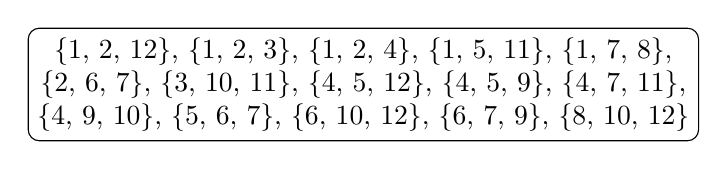
\begin{tikzpicture}[scale=0.7,sibling distance=10em,
  every node/.style = {shape=rectangle, rounded corners,
    draw, align=center}]]
  \node {\{1, 2, 12\}, \{1, 2, 3\}, \{1, 2, 4\}, \{1, 5, 11\}, \{1, 7, 8\},\\\{2, 6, 7\}, \{3, 10, 11\}, \{4, 5, 12\}, \{4, 5, 9\}, \{4, 7, 11\},\\\{4, 9, 10\}, \{5, 6, 7\}, \{6, 10, 12\}, \{6, 7, 9\}, \{8, 10, 12\}};
\end{tikzpicture}
\caption{Initially, all of the hyperedges appear in a single (root) node.}
\label{fig:root-node}
\end{figure}

At every step of the algorithm, we have a valid hypertree decomposition of the input graph.  The algorithm proceeds by moving moving one or more hyperedges from a node to a child node (and possibly creating that child node) at each step.

\subsection{Phase 1}

The algorithm has two phases.  Phase 1 takes a parameter $k$, and attempts to move up to $k$ hyperedges from the root to a child node, then up to $k$ hyperedges from the root to a second child node, and so on.  We only allow a hyperedge to be moved to a child node only if none of its vertices appear in any of the previous child nodes.  Figure \ref{fig:after-phase-1} shows our hypertree decomposition after phase 1, with $k=3$.  Each of the remaining ten hyperedges in the root node shares at least one vertex with a hyperedge in the first child node, and therefore no further moves are possible in this phase.

\begin{figure}
\centering
\scriptsize
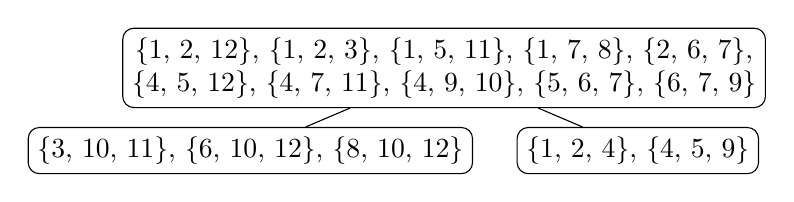
\begin{tikzpicture}[scale=0.7,sibling distance=20em,
  every node/.style = {shape=rectangle, rounded corners,
    draw, align=center}]]
  \node {\{1, 2, 12\}, \{1, 2, 3\}, \{1, 5, 11\}, \{1, 7, 8\}, \{2, 6, 7\},\\\{4, 5, 12\}, \{4, 7, 11\}, \{4, 9, 10\}, \{5, 6, 7\}, \{6, 7, 9\}}
    child {node{\{3, 10, 11\}, \{6, 10, 12\}, \{8, 10, 12\}}}
    child {node{\{1, 2, 4\}, \{4, 5, 9\}}};
\end{tikzpicture}
\caption{The hypertree decomposition after phase 1.  Three hyperedges have been moved from the root into a first child, and two hyperedges have been moved from the root into a second child.  Note that the two children have disjoint vertex sets.}
\label{fig:after-phase-1}
\end{figure}

\subsection{Phase 2}

In phase 2, a small set of rules are followed in order to:
\begin{itemize}
  \item move one or more hyperedges from the root node to a child node created in phase 1, or
  \item create a new child of either the root node or a phase-1 child node, and move one or more hyperedges to the new node from its parent.
\end{itemize}

Figure \ref{fig:after-phase-2} shows the hypertree decomposition after phase 2.
The phase 2 rules are all fairly straightforward, but for brevity we will state only one of them here.  If a node contains a hyperedge $H$ such that every vertex $v \in H$ appears in another of the node's hyperedges, then it safe to create a child node and move $H$ to the child node.  In our running example, this rule was used to create the rightmost node in Figure \ref{fig:after-phase-2}, with the hyperedge $\{5, 6, 7\}$ being moved from the root node.

\begin{figure}[htb]
\centering
\scriptsize
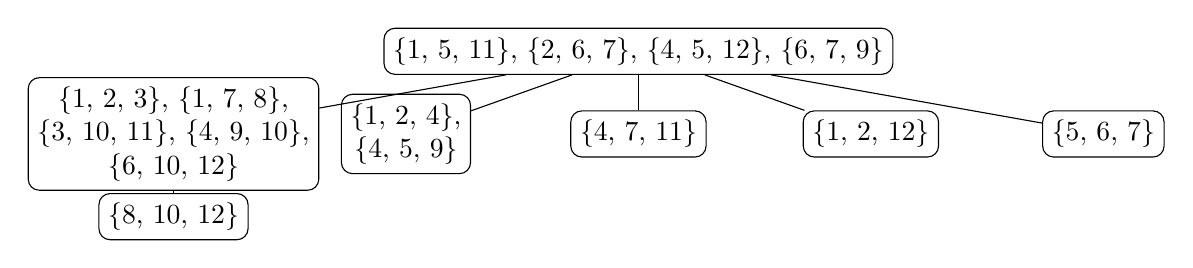
\begin{tikzpicture}[scale=0.7,sibling distance=12em,
  every node/.style = {shape=rectangle, rounded corners,
    draw, align=center}]]
  \node {\{1, 5, 11\}, \{2, 6, 7\}, \{4, 5, 12\}, \{6, 7, 9\}}
    child {node{\{1, 2, 3\}, \{1, 7, 8\},\\\{3, 10, 11\}, \{4, 9, 10\},\\\{6, 10, 12\}}
        child {node{\{8, 10, 12\}}}}
    child {node{\{1, 2, 4\},\\\{4, 5, 9\}}}
    child {node{\{4, 7, 11\}}}
    child {node{\{1, 2, 12\}}}
    child {node{\{5, 6, 7\}}}
    ;
\end{tikzpicture}
\caption{The hypertree decomposition after phase 2.}
\label{fig:after-phase-2}
\end{figure}

%\begin{figure}
%\centering
%\begin{tikzpicture}[sibling distance=10em,
%  every node/.style = {shape=rectangle, rounded corners,
%    draw, align=center}]]
%  \node {\{6, 10, 12\} \{8, 10, 12\} \{3, 10, 11\}}
%    child { node {single-line} }
%    child { node {multi-line}
%      child { node {aligned at}
%        child { node {relation sign} }
%        child { node {several places} }
%        child { node {center} } }
%      child { node {first left,\\centered,\\last right} } };
%\end{tikzpicture}
%\end{figure}

\subsection{Randomness and restarts}

The algorithm is run several hundred times, with the hyperedges being shuffled before each run to give different decompositions.  Furthermore, phase 1 is run with values of $k$ ranging from 1 to one less than the number of hyperedges in the graph.  Finally, the algorithm outputs a decomposition of the smallest width found so far.
}

\end{document}
